%%%%%%%%%%%%%%%%%%%%%%%%%%%%%%%%%%%%%%%%%%%%%%%%%%%%
% Document type, global settings, and packages
%%%%%%%%%%%%%%%%%%%%%%%%%%%%%%%%%%%%%%%%%%%%%%%%%%%%

\documentclass[12pt]{report}   %12 point font for Times New Roman
\usepackage{graphicx}  %for images and plots
\usepackage[letterpaper, left=1.5in, right=1in, top=1in, bottom=1in]{geometry}
\usepackage{setspace}  %use this package to set linespacing as desired
\usepackage{times}  %set Times New Roman as the font
\usepackage[explicit]{titlesec}  %title control and formatting
\usepackage[titles]{tocloft}  %table of contents control and formatting
\usepackage[backend=bibtex, sorting=none, bibstyle=ieee]{biblatex}  %reference manager
\usepackage[bookmarks=true, hidelinks]{hyperref}
\usepackage[page]{appendix}  %for appendices
\usepackage{rotating}  %for rotated, landscape images
\usepackage[normalem]{ulem}  %for italicized text

%%%%%%%%%%%%%%%%%%%%%%%%%%%%%%%%%%%
% Bibliography
%%%%%%%%%%%%%%%%%%%%%%%%%%%%%%%%%%%

%Add your bibliography file here
\bibliography{references}

% prevent certain fields in references from printing in bibliography
\AtEveryBibitem{\clearfield{issn}}
\AtEveryBibitem{\clearlist{issn}}

\AtEveryBibitem{\clearfield{language}}
\AtEveryBibitem{\clearlist{language}}

\AtEveryBibitem{\clearfield{doi}}
\AtEveryBibitem{\clearlist{doi}}

\AtEveryBibitem{\clearfield{url}}
\AtEveryBibitem{\clearlist{url}}

\AtEveryBibitem{%
  \ifentrytype{online}
    {}
    {\clearfield{urlyear}\clearfield{urlmonth}\clearfield{urlday}}}

%%%%%%%%%%%%%%%%%%%%%%
% Start of Document
%%%%%%%%%%%%%%%%%%%%%%

\begin{document}
\doublespacing  %set line spacing

%%%%%%%%%%%%%%%%%%%%%%%%%%%%%%%%%%%%%
% Title Page
%%%%%%%%%%%%%%%%%%%%%%%%%%%%%%%%%%%%%

%% Define your thesis title, your name, your school, and your month and year of graduation here

\newcommand{\thesisTitle}{Object Recognition and Tracking By Deep Learning}
\newcommand{\yourName}{Liqiang Ding}
\newcommand{\yourSchool}{McGill University, Montreal}
\newcommand{\yourMonth}{January}
\newcommand{\yourYear}{2018}

%%%%%%%%%%%%%%%%%%%%%%%%%%%%%%%%%%%%%%%%%%%%%%%%%%%%%%%%%
% Do not edit these lines unless you wish to customize
% the template
%%%%%%%%%%%%%%%%%%%%%%%%%%%%%%%%%%%%%%%%%%%%%%%%%%%%%%%%%



\begin{titlepage}
\begin{center}

\begin{singlespacing}

\textbf{\MakeUppercase{\thesisTitle}}\\
\vspace{10\baselineskip}
\yourName\\
\vspace{3\baselineskip}
Department of Electrical and Computer Engineering\\
McGill University, Montreal\\
\vspace{4\baselineskip}
\yourMonth{} \yourYear{}\\
\vspace{15\baselineskip}
A thesis submitted to the Faculty of Graduate Studies and Research\\
in partial fulfilment of the requirements of the degree of\\
Master of Engineering\\
\vfill
\copyright{} \yourName{} \yourYear{}

\end{singlespacing}

\end{center}
\end{titlepage}



\currentpdfbookmark{Title Page}{titlePage}  %add PDF bookmark for this page

%%%%%%%%%%%%%%%%%%%%%%%%%%%%%%%%%%%%%
% To My Parents
%%%%%%%%%%%%%%%%%%%%%%%%%%%%%%%%%%%%%

% Define your dedication statement here

\newcommand{\yourDedication}{A great dedication goes here.}

%%%%%%%%%%%%%%%%%%%%%%%%%%%%%%%%%%%%%%%%%%%%%%%%%%%%%%%%%
% Do not edit these lines unless you wish to customize
% the template
%%%%%%%%%%%%%%%%%%%%%%%%%%%%%%%%%%%%%%%%%%%%%%%%%%%%%%%%%

\begin{titlepage}
\begin{center}

\vspace*{\fill}
\yourDedication\\
\vspace*{\fill}

\end{center}
\end{titlepage}



\pagenumbering{roman}
\addcontentsline{toc}{chapter}{Abstract}
\setcounter{page}{1} % set the page number appropriately based on the number of intro pages
\addcontentsline{toc}{chapter}{Resume}
\setcounter{page}{2} % set the page number appropriately based on the number of intro pages
\addcontentsline{toc}{chapter}{Acknowledgments}
\setcounter{page}{3} % set the page number appropriately based on the number of intro pages

%%%%%%%%%%%%%%%%%%%%%%%%%%%%%%%%%%%%%
% Abstract
%%%%%%%%%%%%%%%%%%%%%%%%%%%%%%%%%%%%%

\clearpage
\begin{centering}
\vspace{\baselineskip}
\end{centering}

{\LARGE\textbf{Abstract}}
\\
\noindent\rule{15cm}{0.9pt}
\vspace{\baselineskip}

Lorem ipsum dolor sit amet, consectetur adipiscing elit, sed do eiusmod tempor incididunt ut labore et dolore magna aliqua. Ut enim ad minim veniam, quis nostrud exercitation ullamco laboris nisi ut aliquip ex ea commodo consequat. Duis aute irure dolor in reprehenderit in voluptate velit esse cillum dolore eu fugiat nulla pariatur. Excepteur sint occaecat cupidatat non proident, sunt in culpa qui officia deserunt mollit anim id est laborum.


\clearpage
%\pagenumbering{gobble}  %remove page number on summary page


%%%%%%%%%%%%%%%%%%%%%%%%%%%%%%%%%%%%%
% Resume in French
%%%%%%%%%%%%%%%%%%%%%%%%%%%%%%%%%%%%%

\clearpage
\begin{centering}
\textbf{Resume}\\
\vspace{\baselineskip}
\end{centering}

%Insert your dedication text here

\clearpage
%\pagenumbering{gobble}  %remove page number on summary page


%%%%%%%%%%%%%%%%%%%%%%%%%%%%%%%%%%%%%
% Acknowledgments
%%%%%%%%%%%%%%%%%%%%%%%%%%%%%%%%%%%%%

\clearpage
\begin{centering}
\textbf{ACKNOWLEDGEMENTS}\\
\vspace{\baselineskip}
\end{centering}

%Insert your dedication text here
Lorem ipsum dolor sit amet, consectetur adipiscing elit, sed do eiusmod tempor incididunt ut labore et dolore magna aliqua. Ut enim ad minim veniam, quis nostrud exercitation ullamco laboris nisi ut aliquip ex ea commodo consequat. Duis aute irure dolor in reprehenderit in voluptate velit esse cillum dolore eu fugiat nulla pariatur. Excepteur sint occaecat cupidatat non proident, sunt in culpa qui officia deserunt mollit anim id est laborum.

\clearpage
%\pagenumbering{gobble}  %remove page number on summary page


%\addtocontents{toc}{\cftpagenumbersoff{chapter}} 

%\currentpdfbookmark{Acknowledgments}{acknowledgments}
%\addtocontents{toc}{\cftpagenumberson{chapter}} 

%%%%%%%%%%%%%%%%%%%%%%%%%%%%%%%%%%%%%
% Table of Contents
%%%%%%%%%%%%%%%%%%%%%%%%%%%%%%%%%%%%%

% Format for Table of Contents
\renewcommand{\cftchapdotsep}{\cftdotsep}  %add dot separators
\renewcommand{\cftchapfont}{\bfseries}  %set title font weight
\renewcommand{\cftchappagefont}{}  %set page number font weight
\renewcommand{\cftchappresnum}{Chapter }
\renewcommand{\cftchapaftersnum}{:}
\renewcommand{\cftchapnumwidth}{5em}
\renewcommand{\cftchapafterpnum}{\vskip\baselineskip} %set correct spacing for entries in single space environment
\renewcommand{\cftsecafterpnum}{\vskip\baselineskip}  %set correct spacing for entries in single space environment
\renewcommand{\cftsubsecafterpnum}{\vskip\baselineskip} %set correct spacing for entries in single space environment
\renewcommand{\cftsubsubsecafterpnum}{\vskip\baselineskip} %set correct spacing for entries in single space environment

%format title font size and position (this also applys to list of figures and list of tables)
\titleformat{\chapter}[display]
{\normalfont\bfseries\filcenter}{\chaptertitlename\ \thechapter}{0pt}{\MakeUppercase{#1}}

\renewcommand\contentsname{Table of Contents}

\begin{singlespace}
\tableofcontents
\end{singlespace}

\currentpdfbookmark{Table of Contents}{TOC}

\clearpage

%%%%%%%%%%%%%%%%%%%%%%%%%%%%%%%%%%%%%
% List of figures and tables
%%%%%%%%%%%%%%%%%%%%%%%%%%%%%%%%%%%%%

\addcontentsline{toc}{chapter}{LIST OF FIGURES}
\begin{singlespace}
	\setlength\cftbeforetabskip{\baselineskip}  %manually set spacing between entries
	\listoftables
\end{singlespace}

\clearpage

\addcontentsline{toc}{chapter}{LIST OF TABLES}
\begin{singlespace}
\setlength\cftbeforefigskip{\baselineskip}  %manually set spacing between entries
\listoffigures
\end{singlespace}

\clearpage

%%%%%%%%%%%%%%%%%%%%%%%%%%%%%%%%%%%%%%%%%%%%%%%%%%%%%%%%%%%%%%%%%
% This is the Summary (abstract should be separate document)
%%%%%%%%%%%%%%%%%%%%%%%%%%%%%%%%%%%%%%%%%%%%%%%%%%%%%%%%%%%%%%%%%

\clearpage
\begin{centering}
\textbf{SUMMARY}\\
\vspace{\baselineskip}
\end{centering}

Lorem ipsum dolor sit amet, consectetur adipiscing elit, sed do eiusmod tempor incididunt ut labore et dolore magna aliqua. Ut enim ad minim veniam, quis nostrud exercitation ullamco laboris nisi ut aliquip ex ea commodo consequat. Duis aute irure dolor in reprehenderit in voluptate velit esse cillum dolore eu fugiat nulla pariatur. Excepteur sint occaecat cupidatat non proident, sunt in culpa qui officia deserunt mollit anim id est laborum.

%\pagenumbering{gobble}  %remove page number on summary page

%%%%%%%%%%%%%%%%%%%%%%%%%%%%
%
% Chapters
%
%%%%%%%%%%%%%%%%%%%%%%%%%%%%

%%%%%%%%%%%%%%%%%%%%%%
% formatting
%%%%%%%%%%%%%%%%%%%%%%

% resume page numbering for rest of document
\clearpage
\pagenumbering{arabic}
\setcounter{page}{1} % set the page number appropriately

% Adjust chapter title formatting
\titleformat{\chapter}[display]
{\normalfont\bfseries\filcenter}{\MakeUppercase\chaptertitlename\ \thechapter}{0pt}{\MakeUppercase{#1}}  %spacing between titles
\titlespacing*{\chapter}
  {0pt}{0pt}{30pt}	%controls vertical margins on title
  
% Adjust section title formatting
\titleformat{\section}{\normalfont\bfseries}{\thesection}{1em}{#1}

% Adjust subsection title formatting
\titleformat{\subsection}{\normalfont\bfseries}{\thesubsection}{1em}{#1}

% Adjust subsubsection title formatting
\titleformat{\subsubsection}{\normalfont\bfseries}{\thesubsubsection}{1em}{#1}

%%%%%%%%%%%%%%%%
% Chapter 1
%%%%%%%%%%%%%%%%

\chapter{Introduction}

\section{Motivation}

This is a section in Chapter 2.

\section{Thesis Overview}

This is a section in Chapter 2.


% This is a figure
\begin{figure}
	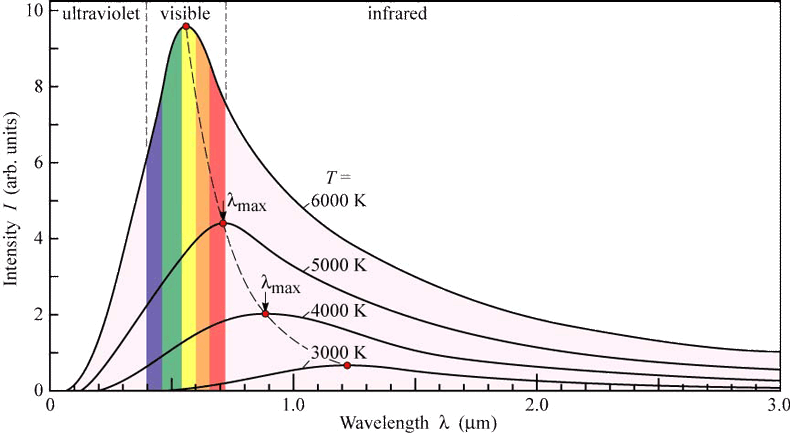
\includegraphics[width=\textwidth]{figures/exampleFigure.png}
	\caption{This is an example Figure.}
	\label{Figure in Chapter 1}
\end{figure}


Lorem ipsum dolor sit amet, consectetur adipiscing elit, sed do eiusmod tempor incididunt ut labore et dolore magna aliqua. Ut enim ad minim veniam, quis nostrud exercitation ullamco laboris nisi ut aliquip ex ea commodo consequat \cite{ref1}. Duis aute irure dolor in reprehenderit in voluptate velit esse cillum dolore eu fugiat nulla pariatur \cite{ref2}. Excepteur sint occaecat cupidatat non proident, sunt in culpa qui officia deserunt mollit anim id est laborum \cite{ref3}.

% This is a table

\begin{table}
\caption{This is an example Table.}
\begin{center}
\begin{tabular}{ccc}
x & f(x) & g(x) \\
\hline
1 & 6 & 4  \\
2 & 6 & 3  \\
3 & 6 & 2  \\
4 & 6 & 2  \\
\label{Table in Chapter 1}
\end{tabular}
\end{center}
\end{table}


%%%%%%%%%%%%%%%%
% Chapter 2
%%%%%%%%%%%%%%%%

\chapter{Previous Approaches}
Lorem ipsum dolor sit amet, consectetur adipiscing elit, sed do eiusmod tempor incididunt ut labore et dolore magna aliqua. Ut enim ad minim veniam, quis nostrud exercitation ullamco laboris nisi ut aliquip ex ea commodo consequat. Duis aute irure dolor in reprehenderit in voluptate velit esse cillum dolore eu fugiat nulla pariatur. Excepteur sint occaecat cupidatat non proident, sunt in culpa qui officia deserunt mollit anim id est laborum.

\section{Section}

This is a section in Chapter 2.

\subsection{Example Subsection}


% This is a figure in landscape orientation
\begin{sidewaysfigure}
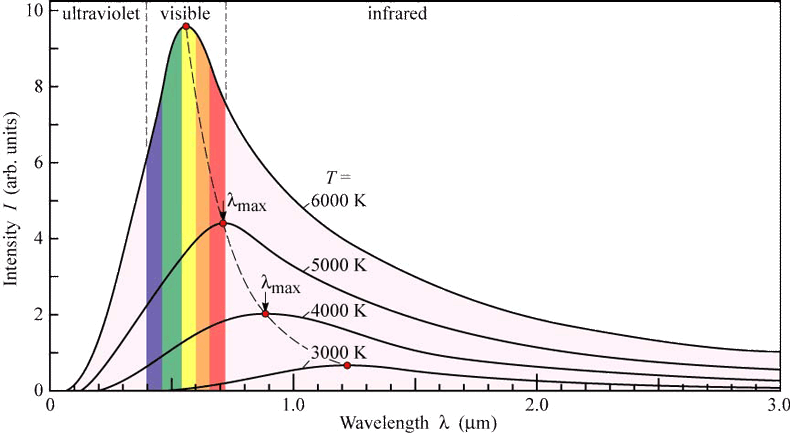
\includegraphics[width=\textwidth]{figures/exampleFigure.png}
\caption{This is another example Figure, rotated to landscape orientation.}
\label{LandscapeFigure}
\end{sidewaysfigure}


%%%%%%%%%%%%%%%%
% Chapter 3
%%%%%%%%%%%%%%%%

\setcounter{secnumdepth}{5}


\chapter{Object Detection and Recognition}

\section{YOLO Darknet}
\subsection{Pre-trained Model with COCO dataset}
\subsection{Trained Model with Customized dataset}
\subsubsection{Dataset}
MIO-TCD\
SPID\
Caltech\
\subsubsection{Kmeans Clustering}
Image clustering 

\section{Neural Network Cascading}
Caltech


%%%%%%%%%%%%%%%%
% Chapter 4
%%%%%%%%%%%%%%%%

\chapter{Object Tracking}

\section{Features}
\subsection{Optical Flow}
\subsubsection{Lucas Kanade Optical Flow Method}
\subsubsection{Farneback Optical Flow Method}
\subsection{Position}
\subsection{Apperance}

\section{Feature Matching}
\subsection{Median Filter}
\subsection{Sample subsubsection}
\subsection{Gaussian Mixture Model}

\section{Kalman Filter Prediction}


%%%%%%%%%%%%%%%%
% Chapter 5
%%%%%%%%%%%%%%%%

\chapter{Experiments and Analysis}
Lorem ipsum dolor sit amet, consectetur adipiscing elit, sed do eiusmod tempor incididunt ut labore et dolore magna aliqua. Ut enim ad minim veniam, quis nostrud exercitation ullamco laboris nisi ut aliquip ex ea commodo consequat. Duis aute irure dolor in reprehenderit in voluptate velit esse cillum dolore eu fugiat nulla pariatur. Excepteur sint occaecat cupidatat non proident, sunt in culpa qui officia deserunt mollit anim id est laborum.


%%%%%%%%%%%%%%%%
% Chapter 6
%%%%%%%%%%%%%%%%

\chapter{Conclusions and Future Work}
Lorem ipsum dolor sit amet, consectetur adipiscing elit, sed do eiusmod tempor incididunt ut labore et dolore magna aliqua. Ut enim ad minim veniam, quis nostrud exercitation ullamco laboris nisi ut aliquip ex ea commodo consequat. Duis aute irure dolor in reprehenderit in voluptate velit esse cillum dolore eu fugiat nulla pariatur. Excepteur sint occaecat cupidatat non proident, sunt in culpa qui officia deserunt mollit anim id est laborum.


%%%%%%%%%%%%%%%%
% Appendices
%%%%%%%%%%%%%%%%

\begin{appendices}

%Some Table of Contents entry formatting
\addtocontents{toc}{\protect\renewcommand{\protect\cftchappresnum}{\appendixname\space}}
\addtocontents{toc}{\protect\renewcommand{\protect\cftchapnumwidth}{6em}}

%Begin individual appendices, separated as chapters

\chapter{Experimental Equipment}
Lorem ipsum dolor sit amet, consectetur adipiscing elit, sed do eiusmod tempor incididunt ut labore et dolore magna aliqua. Ut enim ad minim veniam, quis nostrud exercitation ullamco laboris nisi ut aliquip ex ea commodo consequat. Duis aute irure dolor in reprehenderit in voluptate velit esse cillum dolore eu fugiat nulla pariatur. Excepteur sint occaecat cupidatat non proident, sunt in culpa qui officia deserunt mollit anim id est laborum.

\chapter{Data Processing}
Lorem ipsum dolor sit amet, consectetur adipiscing elit, sed do eiusmod tempor incididunt ut labore et dolore magna aliqua. Ut enim ad minim veniam, quis nostrud exercitation ullamco laboris nisi ut aliquip ex ea commodo consequat. Duis aute irure dolor in reprehenderit in voluptate velit esse cillum dolore eu fugiat nulla pariatur. Excepteur sint occaecat cupidatat non proident, sunt in culpa qui officia deserunt mollit anim id est laborum.

\end{appendices}

%%%%%%%%%%%%%%%%
% References
%%%%%%%%%%%%%%%%

\begin{singlespace}  % use single-line spacing for multi-line text within a single reference
	\setlength\bibitemsep{\baselineskip}  %manually set separataion betwen items in bibliography to double space
	\printbibliography[title={References}]
\end{singlespace}

\addcontentsline{toc}{chapter}{References}  %add References section to Table of Contents

%%%%%%%%%%%%%%%%
% Vita 
% Only for PhD students
% Masters students remove this line
%%%%%%%%%%%%%%%%
\chapter*{Vita}
\addcontentsline{toc}{chapter}{Vita}  %add Vita section to Table of Contents
Vita may be provided by doctoral students only. The length of the vita is preferably one page. It may include the place of birth and should be written in third person. This vita is similar to the author biography found on book jackets.


\end{document}
